% Provenance (never printed): cycle 3 / 6e "La planete Terre" (water in the
% ground, groundwater, springs and wells; resource); see
% sources/book1/PROVENANCE.md. Book 1, grade 6, chapter 5.
% Vocabulary guard: "sediment" not before g7.4; the water cycle is recalled
% from the physics book (prose only).
\chapter{Air di Bawah Tanah}\label{ch:g6:water-underground}

Pada suatu hari yang panas di musim panas, ladang-ladang kering dan
\omterm{def:g1:landscapes-around-us:water}{sungai-sungai} kecil surut. Akan tetapi, di kaki sebuah \omterm{def:g1:landscapes-around-us:landform}{bukit}, air terus
keluar dari tanah, dingin dan jernih, seperti sepanjang musim dingin, dan
mengisi sebuah kolam. Sudah berminggu-minggu \omterm{def:g4:clouds-rain-snow:precipitation}{hujan} tidak turun. Dari mana
air ini berasal, dan bagaimana air itu keluar dari \omterm{def:g3:stones-pebbles-sand:rock}{batuan}?

\begin{omfigure}
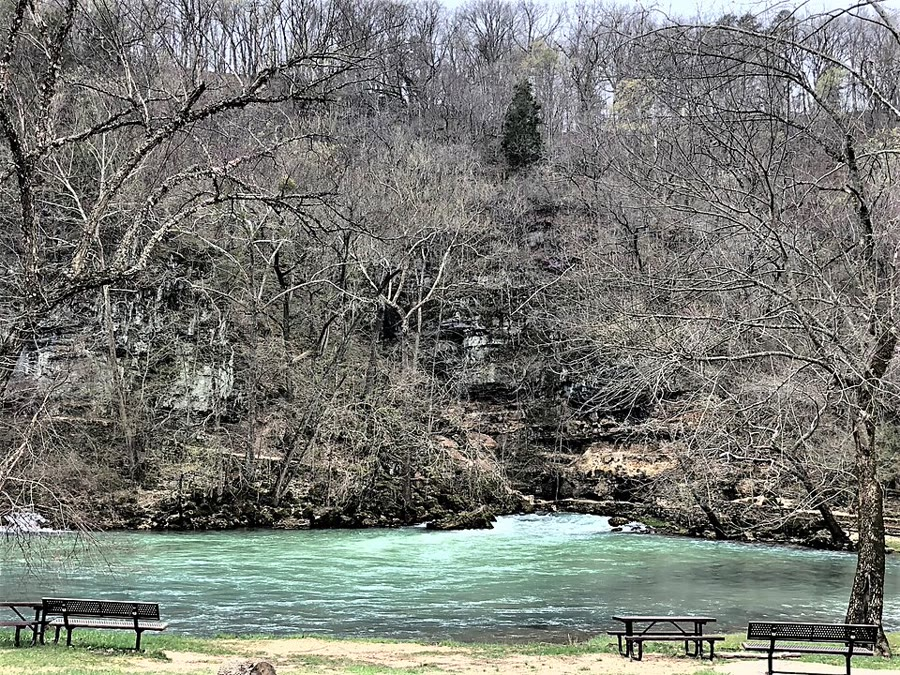
\includegraphics[width=0.72\linewidth]{images/book1/g6-big-spring.jpg}

{\small Sebuah \omterm{def:g6:water-underground:spring}{mata air} muncul di kaki tebing berbatu dan mengisi sebuah
kolam: Big Spring, Missouri (Amerika Serikat). (Foto: Johnston9494, CC BY-SA
4.0, melalui Wikimedia Commons.)}
% ledger: commons:big-spring
\end{omfigure}

\begin{recall}
Hampir semua air di Bumi adalah \omterm{def:g2:water-on-earth:salt-fresh}{air asin}; \omterm{def:g2:water-on-earth:salt-fresh}{air tawar} hanya sebagian kecil,
yang sebagian besar tersimpan sebagai es dan di bawah tanah
(\cref{ch:g2:water-on-earth}). \omterm{def:g3:stones-pebbles-sand:rock}{Batuan} seperti batu pasir dan batu kapur
tersusun dari butiran atau cangkang yang melekat menjadi satu, sedangkan
lempung dan serpih tersusun dari partikel yang sangat halus
(\cref{ch:g6:rocks-and-minerals}). Dalam buku fisika, kamu sudah mengikuti
perjalanan air dalam siklus air: air menguap dari \omterm{def:g2:water-on-earth:ocean}{laut}, mengembun menjadi
\omterm{def:g4:clouds-rain-snow:cloud}{awan}, dan jatuh kembali sebagai \omterm{def:g4:clouds-rain-snow:precipitation}{hujan} atau \omterm{def:g4:clouds-rain-snow:precipitation}{salju}.
\end{recall}

\section{Hujan meresap}

Ketika \omterm{def:g4:clouds-rain-snow:precipitation}{hujan} jatuh di daratan, airnya dapat menempuh tiga jalan. Sebagian
menguap kembali ke udara. Sebagian mengalir di permukaan, menuruni lereng,
masuk ke \omterm{def:g1:landscapes-around-us:water}{sungai-sungai} kecil dan \omterm{def:g1:landscapes-around-us:water}{sungai}: inilah \emph{limpasan}. Sisanya
meresap ke dalam tanah.

\begin{definition}[Infiltrasi]\label{def:g6:water-underground:infiltration}
Yang disebut \emph{infiltrasi}\index{infiltrasi} adalah meresapnya air \omterm{def:g4:clouds-rain-snow:precipitation}{hujan},
atau \omterm{def:g4:clouds-rain-snow:precipitation}{salju} yang mencair, ke dalam tanah, melalui lapisan tanah dan terus ke
bawah masuk ke \omterm{def:g3:stones-pebbles-sand:rock}{batuan}.
\end{definition}

Banyaknya air yang meresap bergantung pada tanahnya. Pada lereng yang
curam, pada tanah yang gundul atau keras, pada jalan atau tempat parkir,
atau ketika tanah sudah basah kuyup, sebagian besar air mengalir pergi. Pada
lereng yang landai, di bawah rumput dan pepohonan, pada tanah berpasir,
lebih banyak air yang sempat meresap.

\begin{omfigure}
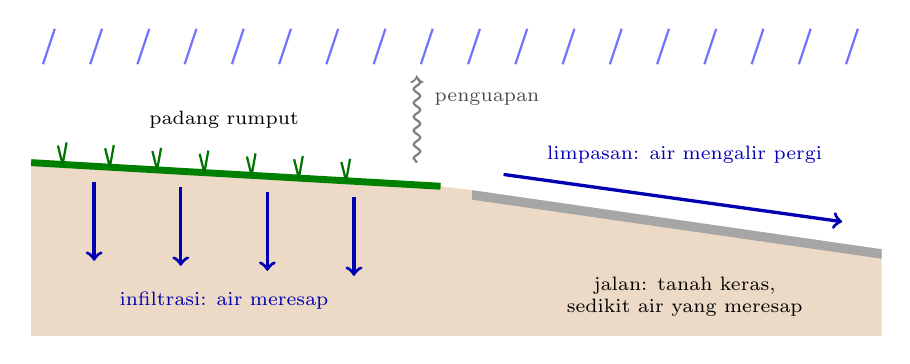
\begin{tikzpicture}[x=1cm, y=1cm]
  % rain
  \foreach \x in {0.3,0.9,...,10.5} \draw[blue!55, thick] (\x,3.9) -- (\x-0.15,3.45);
  % ground: field on the left (gentle), road and town on the right
  \fill[brown!30] (0,0) -- (0,2.2) -- (5.2,1.9) -- (5.6,1.85) -- (10.8,1.1) -- (10.8,0) -- cycle;
  \draw[green!50!black, line width=2.5pt] (0,2.2) -- (5.2,1.9);
  \fill[gray!70] (5.6,1.85) -- (10.8,1.1) -- (10.8,0.98) -- (5.6,1.73) -- cycle;
  \foreach \x in {0.4,1.0,...,4.6} \draw[green!45!black, thick] (\x,{2.2-0.058*\x}) -- ++(0.05,0.28) (\x,{2.2-0.058*\x}) -- ++(-0.06,0.24);
  % infiltration arrows in the field
  \foreach \x in {0.8,1.9,3.0,4.1} \draw[->, blue!70!black, very thick] (\x,{2.0-0.058*\x}) -- ++(0,-1.0);
  \node[font=\scriptsize, blue!70!black, align=center, fill=brown!30] at (2.45,0.45) {infiltrasi: air meresap};
  % run-off on the road
  \draw[->, blue!70!black, very thick] (6.0,2.05) -- (10.3,1.45);
  \node[font=\scriptsize, blue!70!black, align=center] at (8.3,2.3) {limpasan: air mengalir pergi};
  \node[font=\scriptsize, align=center] at (8.3,0.5) {jalan: tanah keras,\\ sedikit air yang meresap};
  \node[font=\scriptsize] at (2.45,2.75) {padang rumput};
  % evaporation
  \draw[->, gray, thick, decorate, decoration={snake, amplitude=1.2pt, segment length=5pt}] (4.9,2.2) -- (4.9,3.3);
  \node[font=\scriptsize, gray!60!black, anchor=west] at (5.0,3.0) {penguapan};
\end{tikzpicture}

{\small Tiga jalan air \omterm{def:g4:clouds-rain-snow:precipitation}{hujan}. Di padang rumput banyak air yang meresap; di
jalan sebagian besar air mengalir pergi.}
\end{omfigure}

\section{Batuan berpori dan permeabel}

Amatilah segenggam \omterm{def:g3:stones-pebbles-sand:sand}{pasir} kering dengan kaca pembesar: di antara
butiran-butirannya ada ruang-ruang kosong yang sangat kecil. Tuangkan air ke
atasnya, dan air itu mengisi ruang-ruang tersebut. Banyak \omterm{def:g3:stones-pebbles-sand:rock}{batuan} yang seperti
itu: penuh dengan lubang kecil di antara butirannya, atau dengan retakan
yang tipis.

\begin{definition}[Porositas]\label{def:g6:water-underground:porosity}
Yang disebut \emph{pori}\index{pori} sebuah \omterm{def:g3:stones-pebbles-sand:rock}{batuan} adalah ruang-ruang kosong
di antara butirannya dan di dalam retakannya. \omterm{def:g3:stones-pebbles-sand:rock}{Batuan} yang mempunyai pori
disebut \emph{berpori}\index{berpori}. Yang disebut
\emph{porositas}\index{porositas} \omterm{def:g3:stones-pebbles-sand:rock}{batuan} adalah bagian volumenya yang berupa
pori, yang dituliskan sebagai persentase.
\end{definition}

\begin{definition}[Permeabilitas]\label{def:g6:water-underground:permeability}
Sebuah \omterm{def:g3:stones-pebbles-sand:rock}{batuan} disebut \emph{permeabel}\index{permeabel} jika air dapat
mengalir melaluinya, karena \omterm{def:g6:water-underground:porosity}{pori-porinya} cukup besar dan saling terhubung.
\omterm{def:g3:stones-pebbles-sand:rock}{Batuan} itu disebut \emph{kedap air}\index{kedap air} jika air tidak dapat
mengalir melaluinya. Yang disebut
\emph{permeabilitas}\index{permeabilitas} adalah seberapa mudah air mengalir
melalui sebuah \omterm{def:g3:stones-pebbles-sand:rock}{batuan}.
\end{definition}

Kedua gagasan ini tidak sama. Lempung sangat \omterm{def:g6:water-underground:porosity}{berpori}: separuh volumenya
berupa \omterm{def:g6:water-underground:porosity}{pori}. Akan tetapi, \omterm{def:g6:water-underground:porosity}{pori-porinya} begitu kecil sehingga air tetap
terperangkap di dalamnya: lempung itu \emph{\omterm{def:g6:water-underground:permeability}{kedap air}}. \omterm{def:g3:stones-pebbles-sand:sand}{Pasir} mempunyai \omterm{def:g6:water-underground:porosity}{pori}
yang lebih sedikit daripada lempung, tetapi \omterm{def:g6:water-underground:porosity}{porinya} lebar dan saling
terhubung: \omterm{def:g3:stones-pebbles-sand:sand}{pasir} itu \emph{\omterm{def:g6:water-underground:permeability}{permeabel}}. Granit yang tidak retak hampir tidak
mempunyai \omterm{def:g6:water-underground:porosity}{pori} sama sekali.
% ledger: heath:porosity

\begin{omfigure}
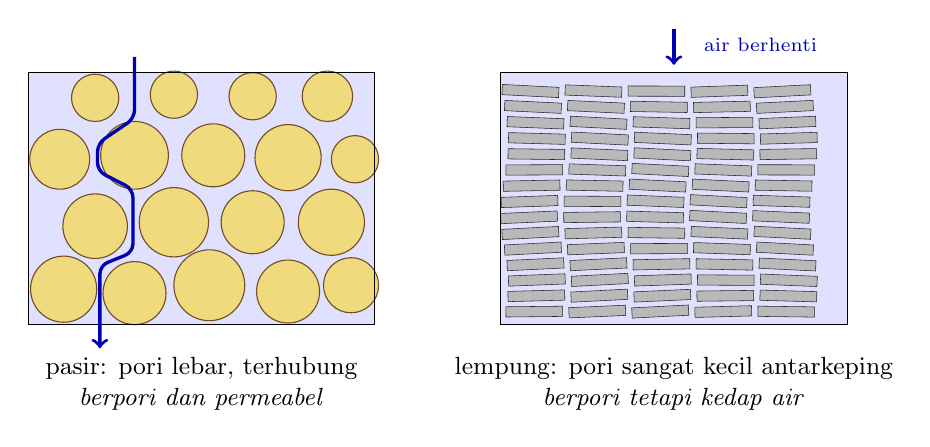
\begin{tikzpicture}
  % sand
  \begin{scope}
    \fill[blue!12] (0,0) rectangle (4.4,3.2);
    \foreach \x/\y/\r in {0.45/0.45/0.42, 1.35/0.4/0.4, 2.3/0.5/0.45, 3.3/0.42/0.4, 4.1/0.5/0.35,
                         0.85/1.25/0.41, 1.85/1.3/0.44, 2.85/1.3/0.4, 3.85/1.3/0.42,
                         0.4/2.1/0.38, 1.35/2.15/0.43, 2.35/2.15/0.4, 3.3/2.12/0.42, 4.15/2.1/0.3,
                         0.85/2.88/0.3, 1.85/2.92/0.3, 2.85/2.9/0.3, 3.8/2.9/0.32}
      \fill[yellow!55!brown!60, draw=brown!60!black] (\x,\y) circle (\r);
    \draw (0,0) rectangle (4.4,3.2);
    \draw[->, blue!70!black, very thick, rounded corners=3pt] (1.35,3.4) -- (1.35,2.62) -- (0.88,2.3) -- (0.88,1.95) -- (1.33,1.72) -- (1.33,0.92) -- (0.91,0.75) -- (0.91,-0.3);
    \node[font=\small, align=center] at (2.2,-0.75) {pasir: pori lebar, terhubung\\ \emph{berpori dan permeabel}};
  \end{scope}
  % clay
  \begin{scope}[xshift=6.0cm]
    \fill[blue!12] (0,0) rectangle (4.4,3.2);
    \foreach \y in {0.1,0.3,...,3.0}
      \foreach \x in {0.05,0.85,...,3.7}
        \fill[gray!55, draw=gray!30!black, line width=0.2pt, rotate around={{3*sin(57*\x+91*\y)}:(\x+0.36,\y+0.06)}]
          ({\x+0.05*sin(200*\y)},\y) rectangle ++(0.72,0.13);
    \draw (0,0) rectangle (4.4,3.2);
    \draw[->, blue!70!black, very thick] (2.2,3.75) -- (2.2,3.3);
    \node[font=\scriptsize, blue!70!black] at (3.3,3.55) {air berhenti};
    \node[font=\small, align=center] at (2.2,-0.75) {lempung: pori sangat kecil antarkeping\\ \emph{berpori tetapi kedap air}};
  \end{scope}
\end{tikzpicture}

{\small \omterm{def:g6:water-underground:porosity}{Pori-pori} (berwarna biru) di antara butiran \omterm{def:g3:stones-pebbles-sand:sand}{pasir} dan di antara
keping-keping lempung, sangat diperbesar. Air menemukan jalan melalui
\omterm{def:g3:stones-pebbles-sand:sand}{pasir}; di dalam lempung, air tetap terperangkap.}
\end{omfigure}

Tabel ini memberikan \omterm{def:g6:water-underground:porosity}{porositas} beberapa bahan, dan bagian air yang keluar
dengan sendirinya dari bahan itu ketika bahan itu penuh berisi air. Sisanya
tetap menempel pada butiran.

\begin{center}\small
\begin{tabular}{|l|c|c|}
\hline
\textbf{bahan} & \textbf{\omterm{def:g6:water-underground:porosity}{porositas} (\%)} & \textbf{air yang keluar (\%)} \\
\hline
tanah & 55 & 40 \\
lempung & 50 & 2 \\
\omterm{def:g3:stones-pebbles-sand:sand}{pasir} & 25 & 22 \\
\omterm{def:g3:stones-pebbles-sand:pebble}{kerikil} & 20 & 19 \\
batu kapur & 20 & 18 \\
batu pasir & 11 & 6 \\
granit & 0.1 & 0.09 \\
\hline
\end{tabular}
\end{center}
% ledger: heath:porosity

\begin{method}[Berapa banyak air yang ditampung sebuah batuan?]\label{met:g6:water-underground:volume}
\begin{enumerate}
  \item Carilah volume \omterm{def:g3:stones-pebbles-sand:rock}{batuan} itu (untuk sebuah balok: panjang $\times$
        lebar $\times$ tinggi).
  \item Kalikan dengan \omterm{def:g6:water-underground:porosity}{porositasnya} dan bagilah dengan 100: hasilnya adalah
        volume \omterm{def:g6:water-underground:porosity}{pori}, jadi air yang ditampung \omterm{def:g3:stones-pebbles-sand:rock}{batuan} itu ketika penuh.
  \item Untuk air yang keluar, pakailah persentase kedua dengan cara yang
        sama. (1~meter kubik sama dengan 1000~liter.)
\end{enumerate}
\end{method}

\begin{example}[Satu meter kubik pasir]\label{ex:g6:water-underground:sand}
Satu meter kubik \omterm{def:g3:stones-pebbles-sand:sand}{pasir}, yang penuh berisi air, menampung $1000 \times 25 \div 100 =
250$~liter air di dalam \omterm{def:g6:water-underground:porosity}{pori-porinya}. Dari jumlah itu, $1000 \times 22 \div 100 = 220$
liter keluar dengan sendirinya; 30~liter tetap menempel pada butiran. Satu
meter kubik lempung menampung air dua kali lebih banyak, 500~liter, tetapi
hanya 20~liter yang keluar.
% ledger: heath:porosity
\end{example}

\begin{inthelab}[Pasir atau lempung? (di kelas, bersama guru)]
Dua pot bunga yang berlubang di dasarnya diletakkan di atas dua gelas. Pot
yang satu diisi \omterm{def:g3:stones-pebbles-sand:sand}{pasir} kering, yang lain diisi tanah lempung kering yang
dipadatkan. Guru menuangkan segelas air yang sama banyaknya ke dalam
masing-masing pot, pada saat yang sama. Melalui \omterm{def:g3:stones-pebbles-sand:sand}{pasir}, air segera menetes ke
dalam gelas di bawahnya. Di atas lempung, air tetap berada di permukaan
sebagai genangan dan hanya beberapa tetes yang keluar, perlahan-lahan: \omterm{def:g3:stones-pebbles-sand:sand}{pasir}
itu \omterm{def:g6:water-underground:permeability}{permeabel}, lempung tidak.
\end{inthelab}

\section{Air tanah dan muka air tanah}

Galilah lubang di \omterm{def:g3:stones-pebbles-sand:sand}{pasir} pantai, beberapa langkah dari \omterm{def:g2:water-on-earth:ocean}{laut}: setelah
beberapa saat, air muncul di dasar lubang. Kamu sudah sampai di tempat yang
semua \omterm{def:g6:water-underground:porosity}{pori} \omterm{def:g3:stones-pebbles-sand:sand}{pasirnya} penuh berisi air.
% ledger: wss:aquifer

\begin{definition}[Air tanah]\label{def:g6:water-underground:groundwater}
Yang disebut \emph{air tanah}\index{air tanah} adalah air di bawah permukaan
tanah yang mengisi \omterm{def:g6:water-underground:porosity}{pori} dan retakan pada tanah dan \omterm{def:g3:stones-pebbles-sand:rock}{batuan}.
\end{definition}

\begin{definition}[Muka air tanah]\label{def:g6:water-underground:water-table}
Di bawah kedalaman tertentu, semua \omterm{def:g6:water-underground:porosity}{pori} \omterm{def:g3:stones-pebbles-sand:rock}{batuan} penuh berisi air. Yang disebut
\emph{muka air tanah}\index{muka air tanah} adalah batas atas zona yang
penuh air ini. Di atasnya, \omterm{def:g6:water-underground:porosity}{pori-pori} berisi udara dan sedikit air; di
bawahnya, \omterm{def:g6:water-underground:porosity}{pori-pori} penuh berisi air.
% ledger: wss:aquifer
\end{definition}

\omterm{def:g6:water-underground:water-table}{Muka air tanah} tidak datar. \omterm{def:g6:water-underground:water-table}{Muka air tanah} mengikuti bentuk daratan, tetapi
lebih landai: lebih tinggi di bawah \omterm{def:g1:landscapes-around-us:landform}{bukit}, lebih rendah di bawah \omterm{def:g1:landscapes-around-us:landform}{lembah}.
\omterm{def:g6:water-underground:water-table}{Muka air tanah} juga naik dan turun mengikuti musim. Setelah musim \omterm{def:g4:clouds-rain-snow:precipitation}{hujan}, air
\omterm{def:g4:clouds-rain-snow:precipitation}{hujan} yang meresap menaikkannya; setelah musim kemarau yang panjang, air
perlahan-lahan mengalir pergi ke \omterm{def:g6:water-underground:spring}{mata air} dan \omterm{def:g1:landscapes-around-us:water}{sungai}, dan \omterm{def:g6:water-underground:water-table}{muka air tanah}
turun.

\omterm{def:g6:water-underground:groundwater}{Air tanah} adalah simpanan \omterm{def:g2:water-on-earth:salt-fresh}{air tawar} yang besar. Dari seluruh \omterm{def:g2:water-on-earth:salt-fresh}{air tawar} di
Bumi, kira-kira 69~\% berupa es dan \omterm{def:g4:clouds-rain-snow:precipitation}{salju} abadi, dan kira-kira 30~\% berupa
\omterm{def:g6:water-underground:groundwater}{air tanah}; \omterm{def:g2:water-on-earth:salt-fresh}{air tawar} di semua \omterm{def:g1:landscapes-around-us:water}{danau} hanya kira-kira seperempat dari satu
persen. \omterm{def:g6:water-underground:groundwater}{Air tanah} lebih dari seratus kali lebih banyak daripada \omterm{def:g2:water-on-earth:salt-fresh}{air tawar} di
\omterm{def:g1:landscapes-around-us:water}{danau-danau}.
% ledger: wss:fresh-shares

\begin{omfigure}
\begin{tikzpicture}
  \begin{axis}[xbar, width=0.8\linewidth, height=3.9cm, bar width=8pt,
      xmin=0, xmax=85, ymin=-0.6, ymax=4.6, y dir=reverse,
      ytick={0,...,4}, yticklabels={es dan salju abadi, air tanah, es tanah dan permafrost, danau, lain-lainnya},
      xlabel={persen dari seluruh air tawar di Bumi},
      axis x line=bottom, axis y line=left, axis line style={-},
      tick label style={font=\scriptsize}, label style={font=\small},
      nodes near coords, nodes near coords style={font=\scriptsize, anchor=west},
      point meta=explicit symbolic, enlarge y limits=false, clip=false]
    \addplot[fill=blue!35, draw=blue!60!black] table[x=pct, y=idx, meta=pct] {figdata/out/grade-6-water_table-fresh.dat};
  \end{axis}
\end{tikzpicture}

{\small Tempat \omterm{def:g2:water-on-earth:salt-fresh}{air tawar} di Bumi berada. Batang untuk \omterm{def:g1:landscapes-around-us:water}{danau} dan untuk
lain-lainnya (\omterm{def:g1:landscapes-around-us:water}{sungai}, udara, tanah, rawa, makhluk hidup) terlalu pendek
untuk terlihat.}
% ledger: wss:fresh-shares (figdata/grade-6/water_table.py, part fresh)
\end{omfigure}

\section{Mata air dan sumur}

\begin{definition}[Mata air dan sumur]\label{def:g6:water-underground:spring}
Yang disebut \emph{mata air}\index{mata air} adalah tempat \omterm{def:g6:water-underground:groundwater}{air tanah} keluar
dari tanah dengan sendirinya, di tempat \omterm{def:g6:water-underground:water-table}{muka air tanah} bertemu dengan
permukaan. Yang disebut \emph{sumur}\index{sumur} adalah lubang yang digali
atau dibor sampai di bawah \omterm{def:g6:water-underground:water-table}{muka air tanah}, sehingga \omterm{def:g6:water-underground:groundwater}{air tanah} mengisi
dasarnya dan dapat diangkat keluar.
\end{definition}

Penampang di bawah ini melintasi sebuah \omterm{def:g1:landscapes-around-us:landform}{lembah} di Perbukitan Varden, wilayah
latihan-latihan kita. Perbukitan itu tersusun dari kapur, sejenis batu kapur
yang putih, lunak, \omterm{def:g6:water-underground:porosity}{berpori}, dan \omterm{def:g6:water-underground:permeability}{permeabel}. Di bawah kapur terdapat lapisan
serpih, yang \omterm{def:g6:water-underground:permeability}{kedap air}. Air \omterm{def:g4:clouds-rain-snow:precipitation}{hujan} meresap ke dalam kapur, mengisi
\omterm{def:g6:water-underground:porosity}{pori-porinya}, dan berhenti di atas serpih.

\begin{omfigure}
\begin{tikzpicture}
\begin{axis}[omsection, width=0.95\linewidth, height=7.2cm,
    xmin=0, xmax=2.8, ymin=0, ymax=560,
    xlabel={jarak dari ujung selatan penampang (km)},
    ylabel={ketinggian di atas permukaan laut (m)},
    tick label style={font=\scriptsize}, label style={font=\small},
    clip mode=individual]
  \addplot[om lith={icsJurassic!40}{om limestone}, draw=black, line width=0.3pt, even odd rule] table {figdata/out/grade-6-water_table-unit-limestone.dat};
  \addplot[om lith={icsJurassic!15}{om shale}, draw=black, line width=0.3pt, even odd rule] table {figdata/out/grade-6-water_table-unit-shale.dat};
  \addplot[om lith={icsCretaceous!35}{om limestone}, draw=black, line width=0.3pt, even odd rule] table {figdata/out/grade-6-water_table-unit-chalk.dat};
  \addplot[lith alluvium, draw=black, line width=0.3pt, even odd rule] table {figdata/out/grade-6-water_table-unit-alluvium.dat};
  \addplot[black, thick] table {figdata/out/grade-6-water_table-ground.dat};
  \addplot[blue!75!black, very thick] table {figdata/out/grade-6-water_table-wet.dat};
  \addplot[blue!75!black, very thick, dashed] table {figdata/out/grade-6-water_table-dry.dat};
  % wells
  \addplot[fill=white, draw=black, line width=0.4pt] table {figdata/out/grade-6-water_table-well-rects.dat};
  \node[font=\scriptsize\bfseries, anchor=south east, fill=white, fill opacity=0.8, text opacity=1, inner sep=1pt] at (axis cs:1.45,401.3) {sumur~A};
  \node[font=\scriptsize\bfseries, anchor=south east, fill=white, fill opacity=0.8, text opacity=1, inner sep=1pt] at (axis cs:1.7,470.3) {sumur~B};
  % river and spring
  \addplot[only marks, mark=*, mark size=2.2pt, blue!75!black] table[x=s_km, y=z_m] {figdata/out/grade-6-water_table-points.dat};
  \node[font=\scriptsize, blue!70!black, anchor=south east] at (axis cs:0.215,140) {sungai};
  \node[font=\scriptsize, blue!70!black, anchor=east] at (axis cs:0.83,218) {mata air};
  \node[font=\scriptsize] at (axis cs:2.2,470) {kapur (permeabel)};
  \node[font=\scriptsize, fill=white, fill opacity=0.8, text opacity=1] at (axis cs:2.2,95) {serpih (kedap air)};
  \node[font=\scriptsize, fill=white, fill opacity=0.8, text opacity=1] at (axis cs:0.95,25) {batu kapur};
  \node[font=\scriptsize, blue!70!black, fill=white, fill opacity=0.8, text opacity=1, align=center] at (axis cs:2.15,250) {muka air tanah:\\ setelah musim hujan (garis penuh)\\ setelah musim kemarau (putus-putus)};
\end{axis}
\end{tikzpicture}

{\small Penampang utara--selatan melalui Perbukitan Varden, dari \omterm{def:g1:landscapes-around-us:water}{sungai} naik
ke lereng \omterm{def:g1:landscapes-around-us:landform}{bukit} sebelah utara (\omterm{def:g4:world-physical-map:altitude}{ketinggian} dibesar-besarkan kira-kira
2~kali). Air yang tersimpan di dalam kapur berhenti di atas serpih dan
keluar sebagai \omterm{def:g6:water-underground:spring}{mata air} di tempat dasar lapisan kapur bertemu dengan
lereng. \omterm{def:g6:water-underground:spring}{Sumur}~A selalu mencapai air; \omterm{def:g6:water-underground:spring}{sumur}~B hanya mencapainya setelah
musim \omterm{def:g4:clouds-rain-snow:precipitation}{hujan}.}
% (figdata/grade-6/water_table.py; region model figdata/shared/region.py)
\end{omfigure}

\omterm{def:g6:water-underground:spring}{Mata air} itu mengalir di tempat dasar lapisan kapur bertemu dengan lereng
\omterm{def:g1:landscapes-around-us:landform}{bukit}: air tidak dapat turun menembus serpih, jadi air mengalir di
sepanjang permukaan atas serpih dan keluar di lereng. Selama masih ada air
di dalam kapur di atas serpih, \omterm{def:g6:water-underground:spring}{mata air} itu terus mengalir, bahkan pada
musim panas yang kering: itulah jawaban atas pertanyaan di awal bab ini.

Perhatikan kedua \omterm{def:g6:water-underground:spring}{sumur} itu. \omterm{def:g6:water-underground:spring}{Sumur}~A sedalam 100~m; dasarnya berada di bawah
\omterm{def:g6:water-underground:water-table}{muka air tanah} pada setiap musim, jadi \omterm{def:g6:water-underground:spring}{sumur} itu selalu memberikan air.
\omterm{def:g6:water-underground:spring}{Sumur}~B bahkan lebih dalam, 105~m, tetapi digali lebih tinggi di \omterm{def:g1:landscapes-around-us:landform}{bukit}:
dasarnya berada di bawah \omterm{def:g6:water-underground:water-table}{muka air tanah} setelah musim \omterm{def:g4:clouds-rain-snow:precipitation}{hujan} dan di atasnya
setelah musim kemarau. Pada musim panas, \omterm{def:g6:water-underground:spring}{sumur}~B mengering. Yang penting
bukanlah seberapa dalam sebuah \omterm{def:g6:water-underground:spring}{sumur}, melainkan seberapa jauh dasarnya
berada di bawah \omterm{def:g6:water-underground:water-table}{muka air tanah} yang paling rendah.
% (figdata/grade-6/water_table.py, part wells)

\begin{omfigure}
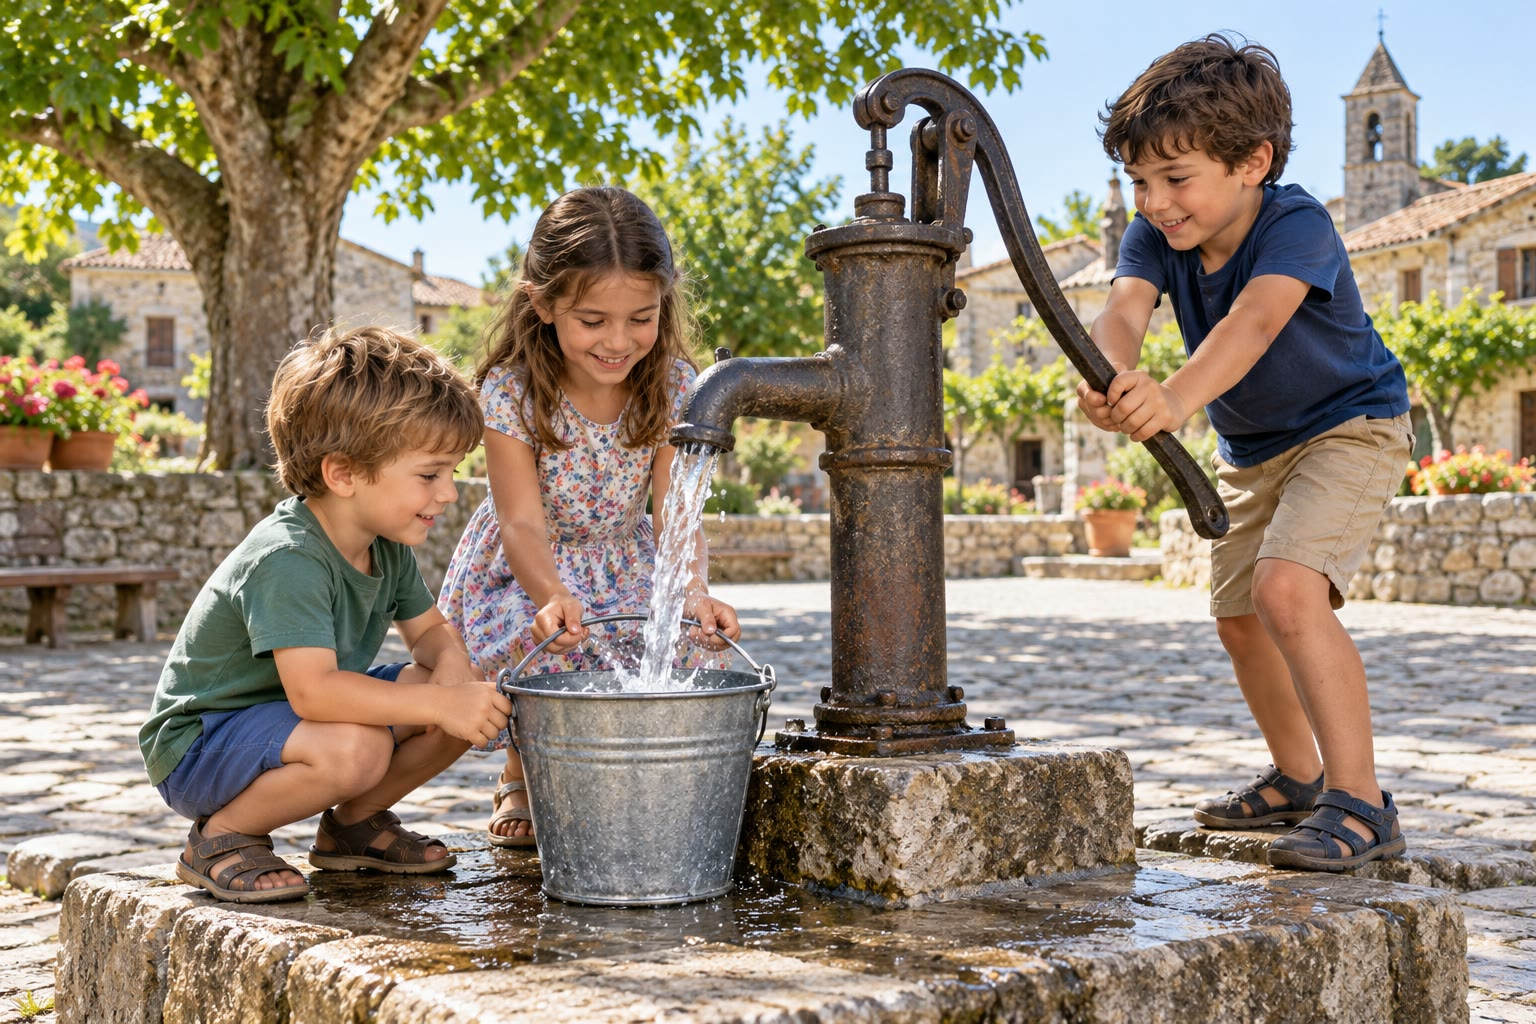
\includegraphics[width=0.6\linewidth]{images/book1/ai/g6-hand-pump.jpg}

{\small Anak-anak mengisi ember di pompa tangan sebuah \omterm{def:g6:water-underground:spring}{sumur} desa.
(Ilustrasi AI.)}
\end{omfigure}

\begin{remark}[Sumur dapat mengering]\label{rem:g6:water-underground:pumping}
Memompa air keluar dari \omterm{def:g6:water-underground:spring}{sumur} menurunkan \omterm{def:g6:water-underground:water-table}{muka air tanah} di sekitarnya. Jika
air dipompa keluar lebih cepat daripada \omterm{def:g4:clouds-rain-snow:precipitation}{hujan} mengisi kembali \omterm{def:g3:stones-pebbles-sand:rock}{batuannya},
\omterm{def:g6:water-underground:water-table}{muka air tanah} terus turun: \omterm{def:g6:water-underground:spring}{sumur} itu memberikan air yang makin lama makin
sedikit dan dapat mengering. Dua tetangga yang memompa dari \omterm{def:g3:stones-pebbles-sand:rock}{batuan} yang sama
berbagi air yang sama: satu pompa dapat mengeringkan \omterm{def:g6:water-underground:spring}{sumur} tetangganya.
% ledger: wss:aquifer
\end{remark}

\section{Akuifer}

\begin{definition}[Akuifer]\label{def:g6:water-underground:aquifer}
Yang disebut \emph{akuifer}\index{akuifer} adalah lapisan \omterm{def:g3:stones-pebbles-sand:rock}{batuan} yang \omterm{def:g6:water-underground:porosity}{berpori}
dan \omterm{def:g6:water-underground:permeability}{permeabel}, yang penuh berisi \omterm{def:g6:water-underground:groundwater}{air tanah}, dan yang membiarkan air ini
mengalir keluar ke \omterm{def:g6:water-underground:spring}{mata air} dan \omterm{def:g6:water-underground:spring}{sumur}. Air \omterm{def:g4:clouds-rain-snow:precipitation}{hujan} yang meresap mengisinya
kembali.
% ledger: wss:aquifer
\end{definition}

Kapur di Perbukitan Varden adalah sebuah \omterm{def:g6:water-underground:aquifer}{akuifer}: kapur itu \omterm{def:g6:water-underground:porosity}{berpori},
\omterm{def:g6:water-underground:permeability}{permeabel}, dan pertanian-pertanian di perbukitan itu mengambil air darinya.
Serpih di bawahnya bukan \omterm{def:g6:water-underground:aquifer}{akuifer}: air tidak dapat mengalir melaluinya. Lebih
dalam lagi, di bawah serpih, terdapat batu kapur dan batu pasir, yang juga
dapat menampung air; untuk mencapai air itu, sebuah \omterm{def:g6:water-underground:spring}{sumur} harus dibor
menembus lapisan serpih.

\omterm{def:g6:water-underground:groundwater}{Air tanah} adalah bagian dari siklus air. \omterm{def:g4:clouds-rain-snow:precipitation}{Hujan} meresap ke dalam \omterm{def:g6:water-underground:aquifer}{akuifer}; \omterm{def:g6:water-underground:groundwater}{air
tanah} mengalir perlahan-lahan melalui \omterm{def:g6:water-underground:porosity}{pori-pori}; air itu keluar di \omterm{def:g6:water-underground:spring}{mata air}
dan masuk ke \omterm{def:g1:landscapes-around-us:water}{sungai}, yang membawanya ke \omterm{def:g2:water-on-earth:ocean}{laut}; di sana air menguap, lalu
jatuh lagi sebagai \omterm{def:g4:clouds-rain-snow:precipitation}{hujan}. Mengambil air dari \omterm{def:g6:water-underground:aquifer}{akuifer} itu seperti mengambil
air dari tangki yang diisi \omterm{def:g4:clouds-rain-snow:precipitation}{hujan} secara perlahan: air itu hanya akan cukup
jika kita tidak mengambil lebih banyak daripada yang dikembalikan \omterm{def:g4:clouds-rain-snow:precipitation}{hujan}.

\section{Menjaga air tanah tetap bersih}

Air yang meresap ke dalam tanah tersaring dalam perjalanannya: daun,
partikel tanah, dan makhluk kecil tertahan oleh tanah dan \omterm{def:g3:stones-pebbles-sand:rock}{batuan}. Itulah
sebabnya air dari \omterm{def:g6:water-underground:spring}{mata air} atau \omterm{def:g6:water-underground:spring}{sumur} biasanya tampak sebening kristal.
Akan tetapi, zat-zat yang \emph{terlarut} di dalam air tidak tertahan: zat
itu ikut turun bersama air sampai ke \omterm{def:g6:water-underground:water-table}{muka air tanah}.
% ledger: wss:gw-quality

\omterm{def:g6:water-underground:groundwater}{Air tanah} dapat tercemar oleh apa yang dibuang manusia ke tanah: pupuk dan
pestisida yang ditebarkan di ladang dan kebun, garam yang ditaburkan di
jalan yang membeku, bahan bakar yang bocor dari tangki, sampah yang dibuang
di tempat terbuka, luapan tangki septik rumah yang tidak terawat. Begitu
terlarut di dalam \omterm{def:g6:water-underground:aquifer}{akuifer}, zat-zat ini sulit dihilangkan, dan airnya mungkin
tidak lagi aman diminum tanpa diolah. Jadi air \omterm{def:g6:water-underground:spring}{sumur} harus diuji sebelum
diminum, dan sebaiknya pupuk, bahan bakar, dan sampah dijauhkan dari \omterm{def:g6:water-underground:spring}{sumur}
dan \omterm{def:g6:water-underground:spring}{mata air}.
% ledger: wss:gw-quality

Zat-zat terlarut berpindah bersama \omterm{def:g6:water-underground:groundwater}{air tanah}. Di bawah \omterm{def:g6:water-underground:water-table}{muka air tanah}, air
merayap perlahan-lahan menuruni lereng: dari tempat \omterm{def:g6:water-underground:water-table}{muka air tanah} tinggi,
di bawah \omterm{def:g1:landscapes-around-us:landform}{bukit}, ke tempat \omterm{def:g6:water-underground:water-table}{muka air tanah} rendah, di \omterm{def:g6:water-underground:spring}{mata air} dan \omterm{def:g1:landscapes-around-us:water}{sungai}.
Karena itu, tumpahan yang meresap tidak tinggal di tempat jatuhnya.
Tumpahan itu turun sampai ke \omterm{def:g6:water-underground:water-table}{muka air tanah}, lalu hanyut menuruni lereng
bersama \omterm{def:g6:water-underground:groundwater}{air tanah}, menuju apa pun yang terletak di bawahnya pada lereng itu.
% ledger: wss:gw-quality, wss:aquifer

\begin{omfigure}
\begin{tikzpicture}[x=1cm, y=1.15cm, font=\scriptsize]
  % ground (the chalk) and the water-filled zone under the water table
  \fill[black!6] (0,0) -- (0,4.090) -- plot[smooth] coordinates {(0.00,4.090) (1.00,4.013) (2.00,3.887) (3.00,3.692) (4.00,3.407) (5.00,3.033) (6.00,2.600) (7.00,2.167) (8.00,1.793) (9.00,1.508) (10.00,1.313) (11.00,1.187) (12.00,1.110)} -- (12,0) -- cycle;
  \fill[blue!14] (0,0) -- (0,3.190) -- plot[smooth] coordinates {(0.00,3.190) (1.00,3.185) (2.00,3.131) (3.00,3.008) (4.00,2.795) (5.00,2.493) (6.00,2.132) (7.00,1.771) (8.00,1.469) (9.00,1.256) (10.00,1.133) (11.00,1.079) (12.00,1.074)} -- (12,0) -- cycle;
  \draw[black!70, line width=0.7pt] plot[smooth] coordinates {(0.00,4.090) (1.00,4.013) (2.00,3.887) (3.00,3.692) (4.00,3.407) (5.00,3.033) (6.00,2.600) (7.00,2.167) (8.00,1.793) (9.00,1.508) (10.00,1.313) (11.00,1.187) (12.00,1.110)};
  \draw[blue!70!black, dashed, line width=0.7pt] plot[smooth] coordinates {(0.00,3.190) (1.00,3.185) (2.00,3.131) (3.00,3.008) (4.00,2.795) (5.00,2.493) (6.00,2.132) (7.00,1.771) (8.00,1.469) (9.00,1.256) (10.00,1.133) (11.00,1.079) (12.00,1.074)};
  % the spill: down to the water table, then downhill with the groundwater
  \fill[brown!70!black, opacity=0.55] (4.85,3.094) -- (5.15,2.971) -- (5.15,2.442) -- (4.85,2.544) -- cycle;
  \fill[brown!70!black, opacity=0.55] (4.85,2.514) -- (5.10,2.429) -- (5.35,2.341) -- (5.60,2.250) -- (5.85,2.158) -- (6.10,2.065) -- (6.35,1.972) -- (6.60,1.881) -- (6.85,1.792) -- (7.10,1.707) -- (7.35,1.626) -- (7.60,1.549) -- (7.85,1.478) -- (8.10,1.413) -- (8.35,1.354) -- (8.60,1.300) -- (8.85,1.252) -- (9.10,1.210) -- (9.30,1.181) -- (9.10,1.182) -- (8.85,1.190) -- (8.60,1.203) -- (8.35,1.221) -- (8.10,1.246) -- (7.85,1.277) -- (7.60,1.313) -- (7.35,1.355) -- (7.10,1.401) -- (6.85,1.486) -- (6.60,1.598) -- (6.35,1.713) -- (6.10,1.828) -- (5.85,1.945) -- (5.60,2.060) -- (5.35,2.174) -- (5.10,2.286) -- (4.85,2.394) -- cycle;
  % the leaking tank
  \draw[fill=black!35] (4.7,3.10) rectangle (5.3,3.42);
  \node[anchor=south, align=center] at (5.0,3.45) {tangki bahan bakar\\yang bocor};
  % groundwater flow
  \begin{scope}[blue!60!black, -{Stealth[length=2mm]}, line width=0.8pt]
    \draw (0.80,2.589) -- (2.40,2.491);
    \draw (3.40,2.334) -- (5.00,1.893);
    \draw (5.90,1.569) -- (7.50,1.009);
    \draw (8.80,0.691) -- (10.60,0.494);
  \end{scope}
  \node[blue!60!black, anchor=north] at (6.7,1.0) {air tanah mengalir menuruni lereng};
  % the two wells
  \draw[line width=1.6pt, black!75] (2.0,3.887) -- (2.0,2.70);
  \draw[line width=1.6pt, black!75] (8.5,1.639) -- (8.5,0.95);
  \node[anchor=south, align=center] at (2.0,3.95) {sumur A\\(di atas): bersih};
  \draw[black!50] (8.5,1.66) -- (8.5,2.30);
  \node[anchor=south, align=center] at (8.5,2.30) {sumur B\\(di bawah): tercemar};
  % the stream
  \fill[blue!60] (11.55,1.13) -- (11.95,1.11) -- (11.75,1.02) -- cycle;
  \node[anchor=south] at (11.6,1.20) {sungai kecil};
  \node[blue!70!black, anchor=south west] at (0.1,3.21) {muka air tanah};
  \node[anchor=west, black!70] at (0.15,0.25) {kapur};
\end{tikzpicture}

{\small Tumpahan di lereng \omterm{def:g1:landscapes-around-us:landform}{bukit} (sketsa). Bahan bakar yang terlarut turun
sampai ke \omterm{def:g6:water-underground:water-table}{muka air tanah}, lalu hanyut menuruni lereng bersama \omterm{def:g6:water-underground:groundwater}{air tanah}
(panah biru): bahan bakar itu mencapai \omterm{def:g6:water-underground:spring}{sumur} B, yang terletak di bawahnya
pada lereng, dan akhirnya \omterm{def:g1:landscapes-around-us:water}{sungai} kecil. \omterm{def:g6:water-underground:spring}{Sumur} A, yang terletak di atas
tangki, tetap bersih.}
\end{omfigure}

\begin{method}[Apakah sebuah sumur terancam?]\label{met:g6:water-underground:risk}
\begin{enumerate}
  \item Carilah tempat \omterm{def:g6:water-underground:water-table}{muka air tanah} tinggi dan tempat \omterm{def:g6:water-underground:water-table}{muka air tanah}
        rendah: \omterm{def:g6:water-underground:water-table}{muka air tanah} tinggi di bawah \omterm{def:g1:landscapes-around-us:landform}{bukit} dan rendah di dekat
        \omterm{def:g6:water-underground:spring}{mata air} dan \omterm{def:g1:landscapes-around-us:water}{sungai}.
  \item \omterm{def:g6:water-underground:groundwater}{Air tanah} mengalir dari tempat yang tinggi ke tempat yang rendah:
        gambarlah arahnya dengan sebuah panah.
  \item \omterm{def:g6:water-underground:spring}{Sumur} atau \omterm{def:g6:water-underground:spring}{mata air} yang terletak di bawah sumber pencemaran, pada
        jalur panah itu, terancam; \omterm{def:g6:water-underground:spring}{sumur} yang terletak di atasnya tidak.
\end{enumerate}
\end{method}

\begin{example}[Tangki bahan bakar baru untuk pertanian]\label{ex:g6:water-underground:tank}
Seorang petani di lereng \omterm{def:g1:landscapes-around-us:landform}{bukit} kapur meminum air dari \omterm{def:g6:water-underground:spring}{sumurnya} sendiri, di
tengah lereng, dan ingin meletakkan tangki bahan bakar baru di salah satu
dari dua ladang: satu di atas \omterm{def:g6:water-underground:spring}{sumur}, satu di bawahnya, dekat \omterm{def:g1:landscapes-around-us:water}{sungai} kecil.
\omterm{def:g6:water-underground:groundwater}{Air tanah} mengalir menuruni lereng. Kebocoran dari ladang di atas akan
hanyut turun menuju \omterm{def:g6:water-underground:spring}{sumur}; kebocoran dari ladang di bawah akan hanyut
menjauhi \omterm{def:g6:water-underground:spring}{sumur}, menuju \omterm{def:g1:landscapes-around-us:water}{sungai} kecil. Ladang di bawah \omterm{def:g6:water-underground:spring}{sumur} adalah pilihan
yang lebih baik bagi \omterm{def:g6:water-underground:spring}{sumur} itu --- dan tangki di atas wadah penampung yang
dapat menahan kebocoran apa pun lebih baik lagi, karena \omterm{def:g1:landscapes-around-us:water}{sungai} kecil itu
juga penting.
\end{example}

\begin{inthefield}[Mencari mata air]
Saat berjalan-jalan bersama orang dewasa, amatilah sepanjang kaki sebuah
lereng. \omterm{def:g6:water-underground:spring}{Mata air} sering kali tampak sebagai sepetak tanah yang basah, sebaris
rumput yang lebih hijau atau alang-alang di ladang yang kering, \omterm{def:g1:landscapes-around-us:water}{sungai} kecil
yang muncul entah dari mana, atau bak batu atau palung yang dibangun untuk
menampung airnya. Pada \omterm{def:g2:drawing-to-map:map}{peta} jalan kaki yang terperinci, \omterm{def:g6:water-underground:spring}{mata air} ditandai
dengan sebuah simbol kecil. Amatilah dari jalan setapak: jangan pernah
meminum air dari \omterm{def:g6:water-underground:spring}{mata air} yang belum diuji.
\end{inthefield}

\section{Latihan}

\begin{exercise}[$\star$]\label{exo:g6:water-underground:1}
Kelompokkan bahan-bahan berikut menjadi ``\omterm{def:g6:water-underground:permeability}{permeabel}'' dan ``\omterm{def:g6:water-underground:permeability}{kedap air}'':
\omterm{def:g3:stones-pebbles-sand:sand}{pasir}, lempung, \omterm{def:g3:stones-pebbles-sand:pebble}{kerikil}, granit yang tidak retak, serpih, kapur.
\end{exercise}

\begin{exercise}[$\star$]\label{exo:g6:water-underground:2}
Pasangkan setiap kata dengan artinya: \omterm{def:g6:water-underground:spring}{mata air}; \omterm{def:g6:water-underground:spring}{sumur}; \omterm{def:g6:water-underground:water-table}{muka air tanah};
\omterm{def:g6:water-underground:aquifer}{akuifer}. (a) Batas atas zona yang semua \omterm{def:g6:water-underground:porosity}{porinya} penuh berisi air.
(b) Lapisan \omterm{def:g6:water-underground:porosity}{berpori} dan \omterm{def:g6:water-underground:permeability}{permeabel} yang menampung \omterm{def:g6:water-underground:groundwater}{air tanah}. (c) Tempat \omterm{def:g6:water-underground:groundwater}{air
tanah} keluar dengan sendirinya. (d) Lubang yang menembus sampai di bawah
\omterm{def:g6:water-underground:water-table}{muka air tanah}.
\end{exercise}

\begin{exercise}[$\star$]\label{exo:g6:water-underground:3}
(a) Sebutkan tiga jalan yang dapat ditempuh air \omterm{def:g4:clouds-rain-snow:precipitation}{hujan} ketika jatuh di
daratan. (b) Setelah \omterm{def:g5:natural-hazards:storm}{badai}, di manakah lebih banyak air yang mengalir pergi:
di tempat parkir atau di padang rumput? Mengapa?
\end{exercise}

\begin{exercise}[$\star$]\label{exo:g6:water-underground:4}
Benar atau salah? Perbaiki kalimat yang salah. (a) \omterm{def:g3:stones-pebbles-sand:rock}{Batuan} yang \omterm{def:g6:water-underground:porosity}{berpori}
selalu \omterm{def:g6:water-underground:permeability}{permeabel}. (b) Di bawah \omterm{def:g6:water-underground:water-table}{muka air tanah}, \omterm{def:g6:water-underground:porosity}{pori-pori} penuh berisi air.
(c) \omterm{def:g6:water-underground:water-table}{Muka air tanah} itu datar, seperti permukaan \omterm{def:g1:landscapes-around-us:water}{danau}. (d) \omterm{def:g2:water-on-earth:salt-fresh}{Air tawar} di
bawah tanah lebih banyak daripada \omterm{def:g2:water-on-earth:salt-fresh}{air tawar} di semua \omterm{def:g1:landscapes-around-us:water}{danau}.
\end{exercise}

\begin{exercise}[$\star\star$]\label{exo:g6:water-underground:5}
Sebuah ember berisi 10~liter \omterm{def:g3:stones-pebbles-sand:sand}{pasir} kering. \omterm{def:g6:water-underground:porosity}{Porositas} \omterm{def:g3:stones-pebbles-sand:sand}{pasir} itu 25~\%.
Berapa banyak air yang dapat kamu tuangkan ke dalam ember sebelum meluap?
Berapa banyak air yang akan keluar melalui lubang di dasarnya (22~\%)?
\end{exercise}

\begin{exercise}[$\star\star$]\label{exo:g6:water-underground:6}
Sebuah balok batu kapur berukuran 2~m kali 1~m kali 1~m. (a) Berapa
volumenya, dalam meter kubik dan dalam liter? (b) \omterm{def:g6:water-underground:porosity}{Porositasnya} 20~\%: berapa
liter air yang ditampungnya ketika penuh? (c) Dari air ini, 18~\% dari
volume balok keluar. Berapa liter yang keluar, dan berapa liter yang tetap
terperangkap?
\end{exercise}

\begin{exercise}[$\star\star$]\label{exo:g6:water-underground:7}
Gunakan penampang melalui Perbukitan Varden. (a) Pada \omterm{def:g4:world-physical-map:altitude}{ketinggian} berapakah
\omterm{def:g6:water-underground:spring}{mata air} itu? \omterm{def:g1:landscapes-around-us:water}{Sungainya}? (b) Apakah \omterm{def:g6:water-underground:spring}{mata air} itu di atas atau di bawah
\omterm{def:g1:landscapes-around-us:water}{sungai}? Ke mana air dari \omterm{def:g6:water-underground:spring}{mata air} itu pergi? (c) Mengapa tidak ada \omterm{def:g6:water-underground:spring}{mata air}
di tengah lereng \omterm{def:g1:landscapes-around-us:landform}{bukit} kapur?
\end{exercise}

\begin{exercise}[$\star\star$]\label{exo:g6:water-underground:8}
Di \omterm{def:g6:water-underground:spring}{sumur}~A, permukaan tanah berada pada 401~m; \omterm{def:g6:water-underground:water-table}{muka air tanah} berada pada
336~m setelah musim \omterm{def:g4:clouds-rain-snow:precipitation}{hujan} dan pada 314~m setelah musim kemarau. (a) Berapa
dalam letak air di bawah permukaan tanah pada setiap musim? (b) Berapa meter
\omterm{def:g6:water-underground:water-table}{muka air tanah} turun di antara kedua musim itu?
\end{exercise}

\begin{exercise}[$\star\star$]\label{exo:g6:water-underground:9}
Seorang petani ingin membuat \omterm{def:g6:water-underground:spring}{sumur} baru di puncak \omterm{def:g1:landscapes-around-us:landform}{bukit}, di ujung kanan
penampang. Haruskah \omterm{def:g6:water-underground:spring}{sumur} itu lebih dalam atau lebih dangkal daripada
\omterm{def:g6:water-underground:spring}{sumur}~A? Jelaskan dengan \omterm{def:g6:water-underground:water-table}{muka air tanah}.
\end{exercise}

\begin{exercise}[$\star\star$]\label{exo:g6:water-underground:10}
Satu meter kubik lempung menampung 500~liter air tetapi hanya memberikan
20~liter. Jelaskan mengapa \omterm{def:g6:water-underground:spring}{sumur} yang digali di dalam lempung hampir tidak
memberikan air, walaupun lempung itu penuh berisi air.
\end{exercise}

\begin{exercise}[$\star\star\star$]\label{exo:g6:water-underground:11}
Dari seluruh \omterm{def:g2:water-on-earth:salt-fresh}{air tawar} di Bumi, 30.1~\% adalah \omterm{def:g6:water-underground:groundwater}{air tanah} dan 0.26~\% berada
di \omterm{def:g1:landscapes-around-us:water}{danau}. (a) Berapa kali lebih banyak \omterm{def:g2:water-on-earth:salt-fresh}{air tawar} di bawah tanah daripada di
\omterm{def:g1:landscapes-around-us:water}{danau}? (b) Dari seluruh \omterm{def:g2:water-on-earth:salt-fresh}{air tawar}, kira-kira 69~\% berupa es dan \omterm{def:g4:clouds-rain-snow:precipitation}{salju}.
Berapa bagian yang tersisa untuk semua yang lain (\omterm{def:g6:water-underground:groundwater}{air tanah}, \omterm{def:g1:landscapes-around-us:water}{danau}, \omterm{def:g1:landscapes-around-us:water}{sungai},
udara, tanah\ldots)? (c) Mengapa \omterm{def:g6:water-underground:groundwater}{air tanah} begitu penting untuk air minum?
\end{exercise}

\begin{exercise}[$\star\star\star$]\label{exo:g6:water-underground:12}
Dua pertanian berdampingan di atas kapur yang sama. Pada suatu musim panas,
pertanian pertama memasang pompa yang kuat dan mengisi sebuah kolam besar;
beberapa minggu kemudian, \omterm{def:g6:water-underground:spring}{sumur} pertanian kedua mengering, walaupun tidak
ada yang menyentuhnya. Jelaskan apa yang terjadi, dan apa yang dapat
dilakukan kedua petani itu.
\end{exercise}

\section{Soal: Sumur Pertanian di Perbukitan Varden}

\begin{problem}[{Soal akhir pekan --- batuan di bawah sebuah pertanian di
Perbukitan Varden, air yang tersimpan di dalam kapurnya, dan berapa hari air
itu akan cukup tanpa hujan}]
\label{pb:g6:water-underground:1}
% ledger: heath:porosity, wss:aquifer
Sebuah pertanian di Perbukitan Varden berdiri di atas kapur, di samping
\omterm{def:g6:water-underground:spring}{sumur}~A pada penampang. Petaninya ingin mengetahui berapa lama \omterm{def:g6:water-underground:spring}{sumur} itu
dapat mencukupi pertanian selama kemarau panjang, jika sama sekali tidak ada
\omterm{def:g4:clouds-rain-snow:precipitation}{hujan} yang mengisi kembali kapur itu.

\medskip
\noindent\textbf{Bagian I --- Batuan di bawah pertanian.}
\begin{enumerate}
  \item Sebutkan \omterm{def:g3:stones-pebbles-sand:rock}{batuan} tempat pertanian itu berdiri, dan \omterm{def:g3:stones-pebbles-sand:rock}{batuan} di
        bawahnya. Manakah yang \omterm{def:g6:water-underground:permeability}{permeabel}?
  \item Jelaskan mengapa ada \omterm{def:g6:water-underground:spring}{mata air} yang mengalir di kaki lereng di bawah
        pertanian itu.
  \item Gunakan penampang: permukaan tanah di pertanian berada pada 401~m
        dan \omterm{def:g6:water-underground:water-table}{muka air tanah} berada pada 336~m setelah musim \omterm{def:g4:clouds-rain-snow:precipitation}{hujan}. Berapa
        dalam letak airnya?
  \item Setelah musim kemarau, \omterm{def:g6:water-underground:water-table}{muka air tanah} berada pada 314~m. \omterm{def:g6:water-underground:spring}{Sumur}~A
        sedalam 100~m. Apakah \omterm{def:g6:water-underground:spring}{sumur} itu masih mencapai air? Berapa meter?
\end{enumerate}

\medskip
\noindent\textbf{Bagian II --- Air di dalam kapur.}
Petani itu dapat mengeringkan kapur di sekitar \omterm{def:g6:water-underground:spring}{sumur} dalam sebuah balok
sepanjang 100~m, selebar 50~m, dan setebal 2~m, di bawah \omterm{def:g6:water-underground:water-table}{muka air tanah}.
Kapur adalah sejenis batu kapur: pakailah \omterm{def:g6:water-underground:porosity}{porositas} 20~\% dan bagian air
yang keluar 18~\%.
\begin{enumerate}[resume]
  \item Berapa volume balok itu, dalam meter kubik?
  \item Berapa meter kubik air yang mengisi \omterm{def:g6:water-underground:porosity}{pori-porinya}?
  \item Berapa meter kubik air yang keluar dari balok itu ke dalam \omterm{def:g6:water-underground:spring}{sumur}?
        Berapa yang tetap terperangkap di dalam kapur?
  \item Tuliskan air yang keluar itu dalam liter.
\end{enumerate}

\medskip
\noindent\textbf{Bagian III --- Berapa lama air itu cukup.}
\begin{enumerate}[resume]
  \item Pertanian itu (rumah, hewan ternak, dan kebun sayur) memakai
        18~meter kubik air setiap hari. Berapa liter itu?
  \item Berapa banyak air yang dipakai pertanian itu dalam seminggu?
  \item Mengapa simpanan air di dalam kapur tidak habis pada tahun yang
        biasa?
  \item Tanpa \omterm{def:g4:clouds-rain-snow:precipitation}{hujan} sama sekali, selama berapa hari air yang keluar dari
        balok itu dapat mencukupi pertanian?
\end{enumerate}
\end{problem}
